% 分离性
% Hausdorff|分离性|正规空间|紧化空间|黎曼球面

\pentry{紧致性\upref{Topo2}}

\subsection{分离性的种类一览}

分离性是描述一个拓扑空间里,任意的点、子集等彼此之间能被不相交的开集分开的程度.我会在这里先列出常见的分离性和它们的简单解释,但你不需要掌握所有分离性,只有其中两个是很重要的.

\begin{definition}{分离性的种类}
\begin{itemize}

\item $T_0$分离性,是指取空间中不同的两点$x,y$,总存在一个开集$U$,使得$U$包含其中一点而不包含另一点.
\item $T_1$分离性,是指取空间中不同的两点$x,y$,总存在两个开集分别含有其中一个点,但各自不含有另一个点.
\item $T_2$分离性,是指取空间中不同的两点$x,y$,总存在两个开集,分别含有其中一个点,并且这两个开集不相交.
\item $T_3$分离性,是指取空间中不同的两点$x,y$或者将$y$替换为一个不含$x$的闭集,那么总存在两个开集,分别含有其中一个点或闭集,并且这两个开集不相交.
\item 正规分离性,是指取空间中不相交的两个闭集$A, B$,总存在两个开集,分别含有其中一个闭集,并且这两个开集不相交.
\item $T_4$分离性,既正规分离又$T_2$分离的性质.


\end{itemize}
\end{definition}

这些分离性之间的区别很细微,看起来很绕,对不对?数学家们将分离性的分类做得比这个要详细得多,除了列表里的,他们还研究了诸如$T_{2.5}$分离性,$T_{3.5}$分离性,$R_1$分离性,完全正规分离性,正则分离性,正则Hausdorff分离性等非常多的分离性.但常用的重要分离性只有其中两个,\textbf{$T_2$分离性}和\textbf{正规分离性}.其中$T_2$分离性又被称为 \textbf{Hausdorff 分离性}.

\subsection{Hausdorff空间和正规空间}

为了方便计,我将重新誊写一遍两个重要分离性的定义.

\begin{definition}{Hausdorff空间和正规空间}
给定拓扑空间$X$.
\begin{itemize}
\item 称$X$是Hausdorff空间,如果任意的$x,y\in X$,都可以被两个不相交的开集$U_x, U_y$分别包含.
\item 称$X$是正规空间,如果任意的两个\textbf{闭集}$A, B\subseteq X$,都可以被两个不相交的开集$U_A, U_B$分别包含.
\end{itemize}
\end{definition}

我们在紧致性\upref{Topo2}一节的开头提到,紧子集的行为常常和单个点是相似的,而紧子集又常常是闭集;在这里,Hausdorff空间和正规空间的概念差别,无非就是一个讨论点和点的关系,另一个讨论闭集和闭集的关系.它们也因此有一些类似的性质.

\begin{theorem}{分离性的继承}
Hausdorff空间的任意子空间还是Hausdorff的.正规空间的任意\textbf{闭}子空间还是正规的.
\end{theorem}

定理证明是很简单的.注意正规空间的继承性要求必须是闭子集构成的空间,因为只有这样才能保证子空间的闭集仍然是原来空间的闭集,从而直接继承原空间的分离性.举个反例,线段$[0,10]$上的度量空间是正规的,如果取子集$(1,3)\cup(4,5)$来构成子空间,那么根据子拓扑的\autoref{Topol_def3}~\upref{Topol},$[2,4]\cap[(1,3)\cup(4,5)]=[2,3)$是$(1,3)\cup(4,5)$空间的闭集,但它显然不是$[0,10]$空间的闭集.当然了,$(1,3)\cup(4,5)$空间也不是正规空间.

紧的Hausdorff空间有一个非常良好的性质:它的紧子集和闭集是等价的.
\begin{theorem}{紧Hausdorff空间的性质}
\begin{itemize}
\item 紧Hausdorff空间的紧子集一定是闭的.
\item 紧Hausdorff空间是正规空间.

\end{itemize}
\end{theorem}

这个定理的证明是非常巧妙的,我列举如下,感兴趣的读者可以仔细体会:

\textbf{证明:}
要证明一个集合是闭集,等价于证明它的补集是开集.

取拓扑空间$X$.设$A$是$X$的紧子集,任取$x\in X-A$.

取$A$中任意一点$a$,由Hausdorff分离性,存在两个开集$U_a\ni a, V_a\ni x$,并且$U_a$和$V_a$不相交.对每一个$a\in A$都取出这样的$U_a$,$V_a$对,那么$\{U_a\}_{a\text{取遍}A}$是$A$的一个覆盖.由于$A$是紧子集,这个覆盖存在有限子覆盖.

也就是说,存在有限个$a_i\in A, i=1, 2, \cdots n$,使得$\{U_{a_i}\}$就足以覆盖$A$了.这里的\textbf{有限}非常关键,因为它使得$\bigcap\limits_{i=1,2, \cdots n}V_{a_i}$是开集的有限交,因此仍然是开集\footnote{回顾拓扑的定义,只要求了任意并和有限交的封闭性;以$\mathbb{R}$为例也可看出,对于所有正整数$n$,开区间$(-1,1/n)$的交集是$(-1, 0]$,这显然不是一个开集.}.

记$\bigcup\limits_{i=1,2, \cdots n}V_{a_i}=U$,且$\bigcap\limits_{i=1,2, \cdots n}V_{a_i}=V$,则$U, V$都是开集,$U\supseteq A$,$V\ni x$,并且$U, V$没有交集$\rightarrow A, V$没有交集.

因此,$x$是$X-A$的一个内点.由于$x$是任意取的,故可知每一个$x\in X-A$都是其内点,故$X-A$是开集,故$A$是闭集.

类似地可以对两个不相交的闭集中的点彼此配对,应用Hausdorff分离性和Hausdorff空间中闭集等价于紧集,可以类似地证明紧Hausdorff空间都是正规空间.


\textbf{证毕.}

\subsection{一点紧化空间}

Hausdorff空间不一定是紧空间,但是总可以添上一个点以后成为紧空间.最常见的例子就是二维平面添上一个点以后成为一个球面,原本的二维平面因为无穷延伸,所以不是紧空间;但是添上一点再相应定义一些新的开集以后,它就等价于一个有限的球面了,从而变成了紧空间.这种添上一点使非紧空间变成紧空间的操作,叫做“一点紧化”.

假设有一个Hausdorff空间$(X, \mathcal{T})$,它不紧致.我给它添上一个点,叫做无穷远点,记为$P$,得到一个新的集合$X\cup \{\mathcal{P}\}=X'$,在这个集合$X'$上定义拓扑:开集一共分两种,含$P$和不含$P$的.不含$P$的开集都是原先$X$中的开集,而含$P$的开集$O$,都是某个$K\subseteq X$的补集:$O=X'-K$.\textbf{其中$K$是$X$的一个紧集}.这样构成了一个新的空间$(X', \mathcal{T}')$,称为$(X, \mathcal{T})$的\textbf{一点紧化空间}.

这样添上一个点并加入和含这个点的开集的定义,就能得到一个紧Hausdorff空间.二维平面变成球面的过程就是这样的.

\begin{example}{黎曼球面}

平面几何所研究的空间$\mathbb{R}^2$是一个Hausdorff空间,但它不紧致——这是很显然的,如果你取$A_n$是以原点为圆心、$n$为半径的圆盘,那么$\{A_n\}$自然是整个平面的一个覆盖,而它不存在有限子覆盖.当我们给这个平面添加一个无穷远点$P$并按照上述方式进行一点紧化以后,所得到的空间实际上等价于一个球面,记为$S^2$.

反过来,你也可以把$\mathbb{R}^2$平面看成是球面$S^2$挖去了一个点$P$构成的.事实上,如果你把一个球放在这个平面的原点处,让球的南极点和原点重合,然后从球的北极点拉出一条条射线穿过球面和平面,球面上和平面上被穿过的点相互联系,就\textbf{几乎}构成了球面和平面的一个双射,\textbf{几乎}每一个球面上的点都唯一对应平面上的一个点,除了北极点本身.这个北极点就是我们所讨论的$P$点,那个在平面上并不存在的无穷远点.

\begin{figure}[ht]
\centering
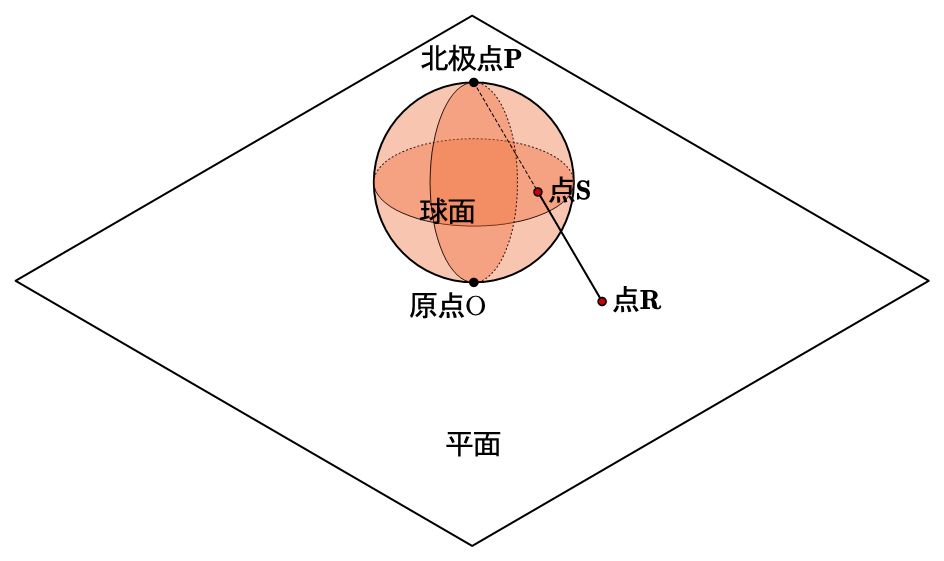
\includegraphics[width=10cm]{./figures/Topo5_1.png}
\caption{黎曼球面示意图.图中球面的南极点和平面的原点$O$是重合的.从北极点$P$拉出的一条射线在$S$穿过球面,和平面相交于$R$.球面和平面上的各点$S$和$R$以这种方式一一对应.} \label{Topo5_fig1}
\end{figure}

这样给$\mathbb{R}^2$平面添上一个无穷远点并定义新的开集以后所得到的球面,被称为\textbf{黎曼球面}.通常我们会规定这个球面半径为$1$.
\end{example}



